% ----------------------------------------------------------
% Chapter 1
% ----------------------------------------------------------
\chapter{Introduction}
% ----------------------------------------------------------

Concurrency is an attribute of any system that allows multiple components to perform operations at the same time. The understanding of this property is essential in modern programming because major areas, such as distributed and real-time systems, rely on this concept to work properly. As a result, the variety of applications enabled by the concurrency feature is broad: aircraft and industrial control systems, routing algorithms, peer-to-peer networks, client-server applications and parallel computation, to name a few.

Since concurrent systems may have parts that execute in parallel, the combination of ways in which these parts can interact raises the complexity in designing such systems. Phenomena like deadlock, livelock, nondeterminism and race condition can emerge from these interactions, so these issues must be addressed in order to avoid undesired behaviour. Typically, testing cannot provide enough evidence to guarantee properties such as deadlock freedom, divergence freedom and determinism for a given system.

That being said, CSP, a theory for Communicating Sequential Processes, introduces a convenient notation that allows concurrent systems to be described in a clear and accurate way. More than that, it has an underlying theory that enables designs to be analysed and proven correct with respect to desired properties. The FDR (Failures-Divergence Refinement) tool is a refinement (model) checker for CSP responsible for making this process algebra a practical tool for specification, analysis and verification of systems. System analysis is achieved by allowing the user to make assertions about processes and then exploring every possible behavior, if necessary, to check the truthfulness of the assertions made.

Although it is undeniable that FDR is a useful tool in the analysis of systems described in CSP, it has a limitation that is common to standard model checkers in general: the state explosion problem. An alternative way for deciding whether a system meets its specification is by proof development. Examples of this different approach are CSP-Prover~\cite{Roggenbach:CSP-Prover} and Isabelle/UTP~\cite{Woodcock:Isabelle/UTP}, both frameworks based on the theorem prover Isabelle. Nevertheless, to the best of our knowledge, there is not a theory for CSP in the Coq proof assistant yet \cite{bertot:coq}. Considering that, the main research question of this work is the following: how could we develop a theory for CSP in Coq, exploiting the main advantages of this proof assistant?

% ---
\section{Objectives}
% ---

The main objective (MO) of this work is to define in Coq a theory for concurrent systems, based on a limited scope of the process algebra CSP. This objective is unfolded into the following specific objectives (SO):

\begin{itemize}
	\item SO1: study CSP and frameworks based on this process algebra.
	\item SO2: define a syntax for CSP in Coq, based on a restricted version of the \CSPM{} language (machine readable language for CSP).
	\item SO3: provide support for the LTS-based (Labelled Transition System) representation, considering the Structured Operational Semantics (SOS) of CSP.
	\item SO4: make use of the QuickChick tool to search for counterexamples of the traces refinement relation.
\end{itemize}

% ---
\section{An overview of \CSPcoq{}}
% ---

To illustrate \CSPcoq{}, our dialect of CSP in Coq, consider the following CSP process, which has been adapted from \citeonline[p.~32, example 2.3]{schneider1999}. This process represents a cloakroom attendant that might help a costumer off or on with his coat, storing and retrieving coats as appropriate.
%
\begin{align}
	\mathit{channel\ coat\_on, coat\_off, store, retrieve, request\_coat, eat}\notag
\end{align}
\begin{align}
	\mathit{SYSTEM} =\ &\mathit{coat\_off \mathbin{{-}{>}} store \mathbin{{-}{>}} request\_coat \mathbin{{-}{>}} retrieve \mathbin{{-}{>}} coat\_on \mathbin{{-}{>}} SKIP}\notag\\
			 &[|\ \{\mathit{coat\_off, request\_coat, coat\_on}\}\ |]\notag\\
	  		 &\mathit{coat\_off \mathbin{{-}{>}} eat \mathbin{{-}{>}} request\_coat \mathbin{{-}{>}} coat\_on \mathbin{{-}{>}} SKIP}\notag
\end{align}

The system comprises six possible events (\emph{coat\_on}, \emph{coat\_off}, among others), and its behaviour is described by the parallel synchronisation of the attendant's and the costumer's behaviours, requiring that they need to synchronise on the execution of the following events: \emph{coat\_off}, \emph{request\_coat}, and \emph{coat\_on}. Regarding the other events, the attendant and the costumer are free to perform them as they wish.

We can declare such system in \CSPcoq{} by defining a specification, which consists of lists of channels and processes. This specification must also abide by a set of contextual rules that will be discussed further in this work.

\begin{coqdoccode}
	\coqdocnoindent
	\coqdockw{Definition} \coqdocvar{example} : \coqdocvar{specification}.\coqdoceol
	\coqdocnoindent
	\coqdockw{Proof}.\coqdoceol
	\coqdocindent{1.00em}
	\coqdocvar{solve\_spec\_ctx\_rules} (\coqdoceol
	\coqdocindent{2.00em}
	\coqdocvar{Build\_Spec}\coqdoceol
	\coqdocindent{2.00em}
	[ \coqdocvar{Channel} \{\{``coat\_off'', ``coat\_on'', ``request\_coat'', ``retrieve'', ``store'', ``eat''\}\} ]\coqdoceol
	\coqdocindent{2.00em}
	[ ``SYSTEM'' ::=\coqdoceol
	\coqdocindent{3.00em}
	``coat\_off'' -{}-> ``store'' -{}-> ``request\_coat'' -{}-> ``retrieve'' -{}-> ``coat\_on'' -{}-> \coqdocvar{SKIP}\coqdoceol
	\coqdocindent{3.00em}
	[| \{\{``coat\_off'', ``request\_coat'', ``coat\_on''\}\} |]\coqdoceol
	\coqdocindent{3.00em}
	``coat\_off'' -{}-> ``eat'' -{}-> ``request\_coat'' -{}-> ``coat\_on'' -{}-> \coqdocvar{SKIP} ]\coqdoceol
	\coqdocindent{1.00em}
	).\coqdoceol
	\coqdocnoindent
	\coqdockw{Defined}.\coqdoceol
\end{coqdoccode}

As one can see, the main syntax of \CSPcoq{} is close that of \CSPM{}. It is also important to emphasise that the tactic \emph{solve\_spec\_ctx\_rules} proves the aforementioned contextual rules with no user intervention (automatically). Furthermore, we can execute the following command to compute the process LTS and output the corresponding graph in the dot language:

\begin{coqdoccode}
	\coqdocnoindent
	\coqdockw{Compute} \coqdocvar{generate\_dot} (\coqdocvar{compute\_ltsR} \coqdocvar{example} ``SYSTEM'' 100).\coqdoceol
\end{coqdoccode}

\autoref{lts-example} is a visual representation of the graph outputted by this command. The image is generated using the GraphViz software. The red circle denotes the starting node, and the edges are labelled by the performed events.

\begin{figure}[htb]
	\caption[The LTS for the cloakroom example]{The LTS for the cloakroom example}
	\label{lts-example}
	\begin{center}
		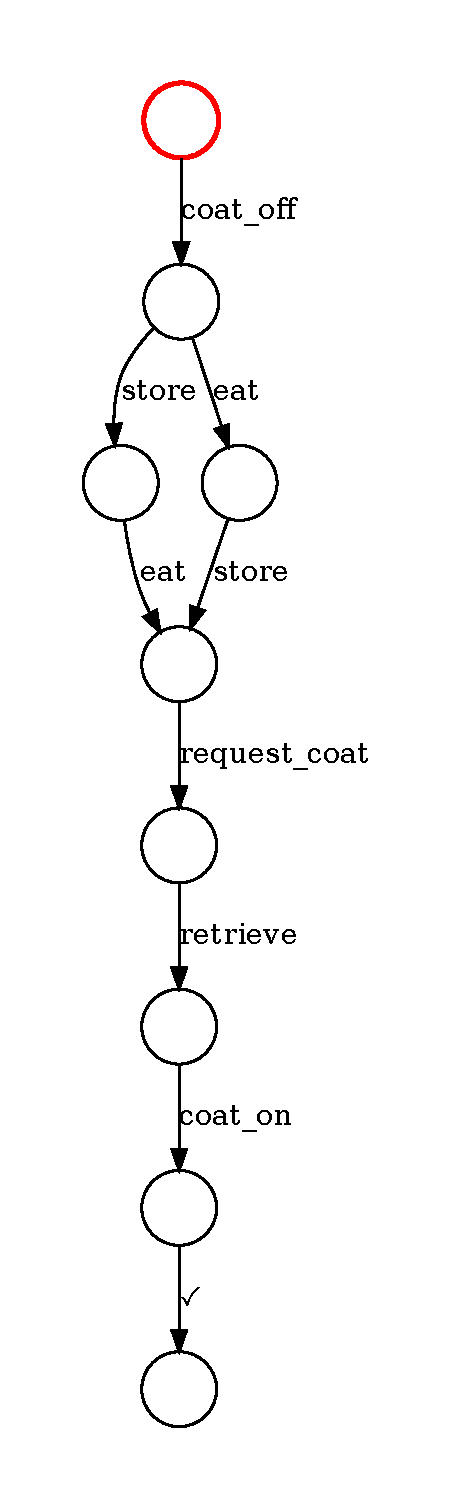
\includegraphics[scale=0.5]{images/LTS.pdf}
	\end{center}
\end{figure}

% ---
\section{Main contributions}
% ---

The main contribution of this work is an initial formalisation of CSP in Coq (\CSPcoq{}), which takes into account the following aspects:

\begin{itemize}
	\item Abstract and concrete syntaxes for a subset of CSP operators.
	\item Contextual rules for CSP specifications.
	\item Proof automation for checking contextual rules.
	\item Operational semantics via the SOS approach.
	\item Inductive and functional definitions of labelled transition systems.
	\item Inductive and functional definitions of traces.
	\item Proof automation for checking whether a list of events is a valid trace.
	\item Formal definition of traces refinement.
	\item Traces refinement verification using QuickChick.
\end{itemize}

% ---
\section{Document structure}
% ---

Apart from this introductory chapter, in which we discuss about the motivation behind this work and its main objective, and also takes a quick look at an example that illustrates what can be done using the framework developed, this monograph contains three more chapters. The content of these chapters are detailed below:

\begin{description}
	\item [Chapter 2] Discusses fundamental concepts such as the CSP theory, the SOS approach, trace refinement and LTS representation. Additionally, this chapter introduces the Coq proof assistant and its functional language Gallina, along with an introduction to proof development (tactics) and the Ltac language, which gives support for proof automation.
	\item [Chapter 3] Provides an in-depth look at the implementation of \CSPcoq{}, including its abstract and concrete syntaxes, in addition to the language semantics. Furthermore, the support for visualising processes as LTSs, using the GraphViz software, is also detailed in this chapter.
	\item [Chapter 4] Concludes this monograph by presenting a comparison between the infrastructure described in this work and related solutions based on other interactive theorem provers. It also addresses possible topics for future work.
\end{description}